\documentclass[..\uwthesis.tex]{subfiles}
\begin{document}


\chapter{Supplementary material for O'Brien et al. 2019}

% TABLE S1 - CORRELATIONS WITH READING SKILL
\begin{table}
\centering
\caption{Correlations with composite reading score}
\label{tab:sb_rdcorr}
    \begin{tabular}{lrrl}
    \toprule
     Measure & $\beta$ & SE & $p$\\
    \midrule
    Age                & 1.08 & 1.40 & 0.443\\
    ADHD diagnosis     & -6.91 & 4.45 & 0.124\\
    Gender             & 1.01 & 3.78 & 0.780\\
    \textbf{CTOPP-2} &  &  &  \\
    Phonological Awareness & 0.65 & 0.11 & $< 0.001$\\
    Phonological Memory &0.57 & 0.10 & $< 0.001$\\
    Rapid Automatic Naming & 0.88 & 0.08 & $< 0.001$\\
    \textbf{TOWRE-2} & & & \\
    Pseudoword Decoding & 1.02 & 0.03 & $< 0.001$\\
    Sight Word Reading & 0.82 & 0.03 & $< 0.001$\\
    \textbf{WASI-II} & & & \\
    Full-scale IQ & 0.75 & 0.09 & $< 0.001$\\
    Matrix Reasoning & 0.95 & 0.16 & $< 0.001$\\
    Vocabulary & 0.97 & 0.13 & $< 0.001$\\
    \textbf{Woodcock Johnson IV} & & & \\
    Letter Word Identification & 0.91 & 0.03 & $< 0.001$\\
    Word Attack & 0.94 & 0.05 & $< 0.001$\\
     
    \bottomrule
    \end{tabular}
\end{table}

% TABLE S2 - GROUP DEMOGRAPHICS
\begin{table}
  \begin{threeparttable}
    \caption{Group demographic measures}
    \label{tab:sb_group_demo}
    \begin{tabular}{llll}
    \toprule
      & Control & Dyslexic & Significance\\
    \midrule
     & $n=$48 & $n=$43 & \\
     & 28 male, 20 female & 25 male, 18 female & \\
    \textbf{CTOPP 2} &  &  & \\
    Phonological Awareness & 98.3 (15.0) & 86.4 (12.7) & $<0.001$\\
    Phonological Memory & 98.6 (17.3) & 84.9 (12.8) & $<0.001$\\
    Rapid Naming & 99.4 (12.5) & 79.0 (9.6) & $<0.001$\\
    \textbf{TOWRE 2} &  &  & \\
    TOWRE Index & 106.8 (11.0) & 68.4 (8.0) & $<$ 0.001\\
    Pseudoword Decoding & 104.6 (11.4) & 71.6 (6.3) & $<$ 0.001\\
    Sight Word Efficiency & 108.2 (11.7) & 68.5 (11.3) & $<$ 0.001\\
    \textbf{WASI-III} &  &  & \\
    Full-scale IQ & 115.8 (16.0) & 96.3 (9.9) & $<$ 0.001\\
    Matrix Reasoning & 55.3 (10.8) & 46.6 (7.3) & $<$ 0.001\\
    Vocabulary & 63.2 (11.0) & 49.1 (7.8) & $<0.001$\\
    \textbf{Woodcock-Johnson IV} &  &  & \\
    Basic Reading Score & 110.3 (12.7) & 77.2 (10.5) & $<$ 0.001\\
    Letter Word Identification & 109.8 (11.8) & 74.4 (12.1) & $<$ 0.001\\
    Word Attack & 109.4 (14.9) & 82.4 (10.8) & $<$ 0.001\\


    \bottomrule
\end{tabular}
    \end{threeparttable}
\end{table}




% TABLE S3 - PARAMETER RELIABILITY
\begin{table}
\caption{DDM parametr reliability estimates}
\label{tab:sb_reliability}
\centering
    \begin{tabular}{lrrl}
    \toprule
    \multicolumn{1}{c}{} & \multicolumn{1}{c}{} & \multicolumn{1}{c}{} \\
    \makecell[c]{Parameter} & \makecell[c]{Split-half\\reliability} & \makecell[c]{Adjusted\\reliability}\\
    \midrule
    $v_6$ & 0.093 & 0.170 \\
    $v_{12}$ & 0.397 & 0.568 \\
    $v_{24}$ & 0.353 & 0.522 \\
    $v_{48}$ & 0.512 & 0.677 \\
    $a$ & 0.531 & 0.693 \\
    $t$ & 0.594 & 0.737 \\
    $sv$ & 0.141 & 0.248 \\
    $sz$ & 0.279 & 0.436 \\
    \bottomrule
    \end{tabular}
\item \textit{Split half reliability is calculated by partitioning each subject’s responses into two by random assignment, estimating the DDM parameters on each half, and measuring the Pearson’s correlation between parameter estimates. Adjusted reliability is calculated with the Spearman-Brown prophecy formula. This adjustment is an estimate of the reliability had the estimates been computed on twice as many observations as in split-half reliability. }
\end{table}

%TABLE S4 - SELECTED MODEL OR REACTION TIME ON MOTION DISCRIMIN TASK
\begin{table}
\centering
\caption{Selected model of reaction time on the motion discrimination task}
\label{tab:sb_rtmodel}
    \begin{tabular}{lrrl}
    \toprule
      & $\beta$ & SE & $p$\\
    \midrule
    (Intercept)   & 4.101  & 0.316 & $<$ 0.001\\
    Coherence     & -0.173 & 0.009 & $<$ 0.001\\
    Age           & -0.059 & 0.021 & 0.007\\
    Reading skill & -0.006 & 0.001 & $<$ 0.001 \\
    \bottomrule
    \end{tabular}
\end{table}

%TABLE S5 - SELECTED MODEL OF ACCURACY ON MOTION DISCRIMIN TASK
\begin{table}
\centering
\caption{Selected model of accuracy on the motion discrimination task}
\label{tab:sb_accmodel}
    \begin{tabular}{lrrl}
    \toprule
      & $\beta$ & SE & $p$\\
    \midrule
    (Intercept)   & 0.218 & 0.062 & $<$ 0.001\\
    Coherence     & 0.084 & 0.003 & $<$ 0.001\\
    Age           & 0.024 & 0.006 & $<$ 0.001\\
    \bottomrule
    \end{tabular}
\end{table}

%TABLE S6 - SELECTED MODEL OF ACCURACY ON MOTION DISCRIMIN TASK
\begin{table}
\centering
\caption{Selected model of the ratio of error-to-correct reponse times on the motion discrimination task.}
\label{tab:sb_ratio}
    \begin{tabular}{lrrl}
    \toprule
      & $\beta$ & SE & $p$\\
    \midrule
    (Intercept)      & 0.555  & 0.350 & 0.115\\
    Reading skill    & 0.004  & 0.002 & 0.050\\
    Age              & 0.080  & 0.028 & 0.005\\
    Nonverbal IQ     & -0.007 & 0.004 & 0.096\\
    \bottomrule
    \end{tabular}
\end{table}



% FIGURE 1
\begin{figure}
    \centering
    \caption{Reaction times and accuracy on random dot motion task.}
    \label{fig:suppb_1}
    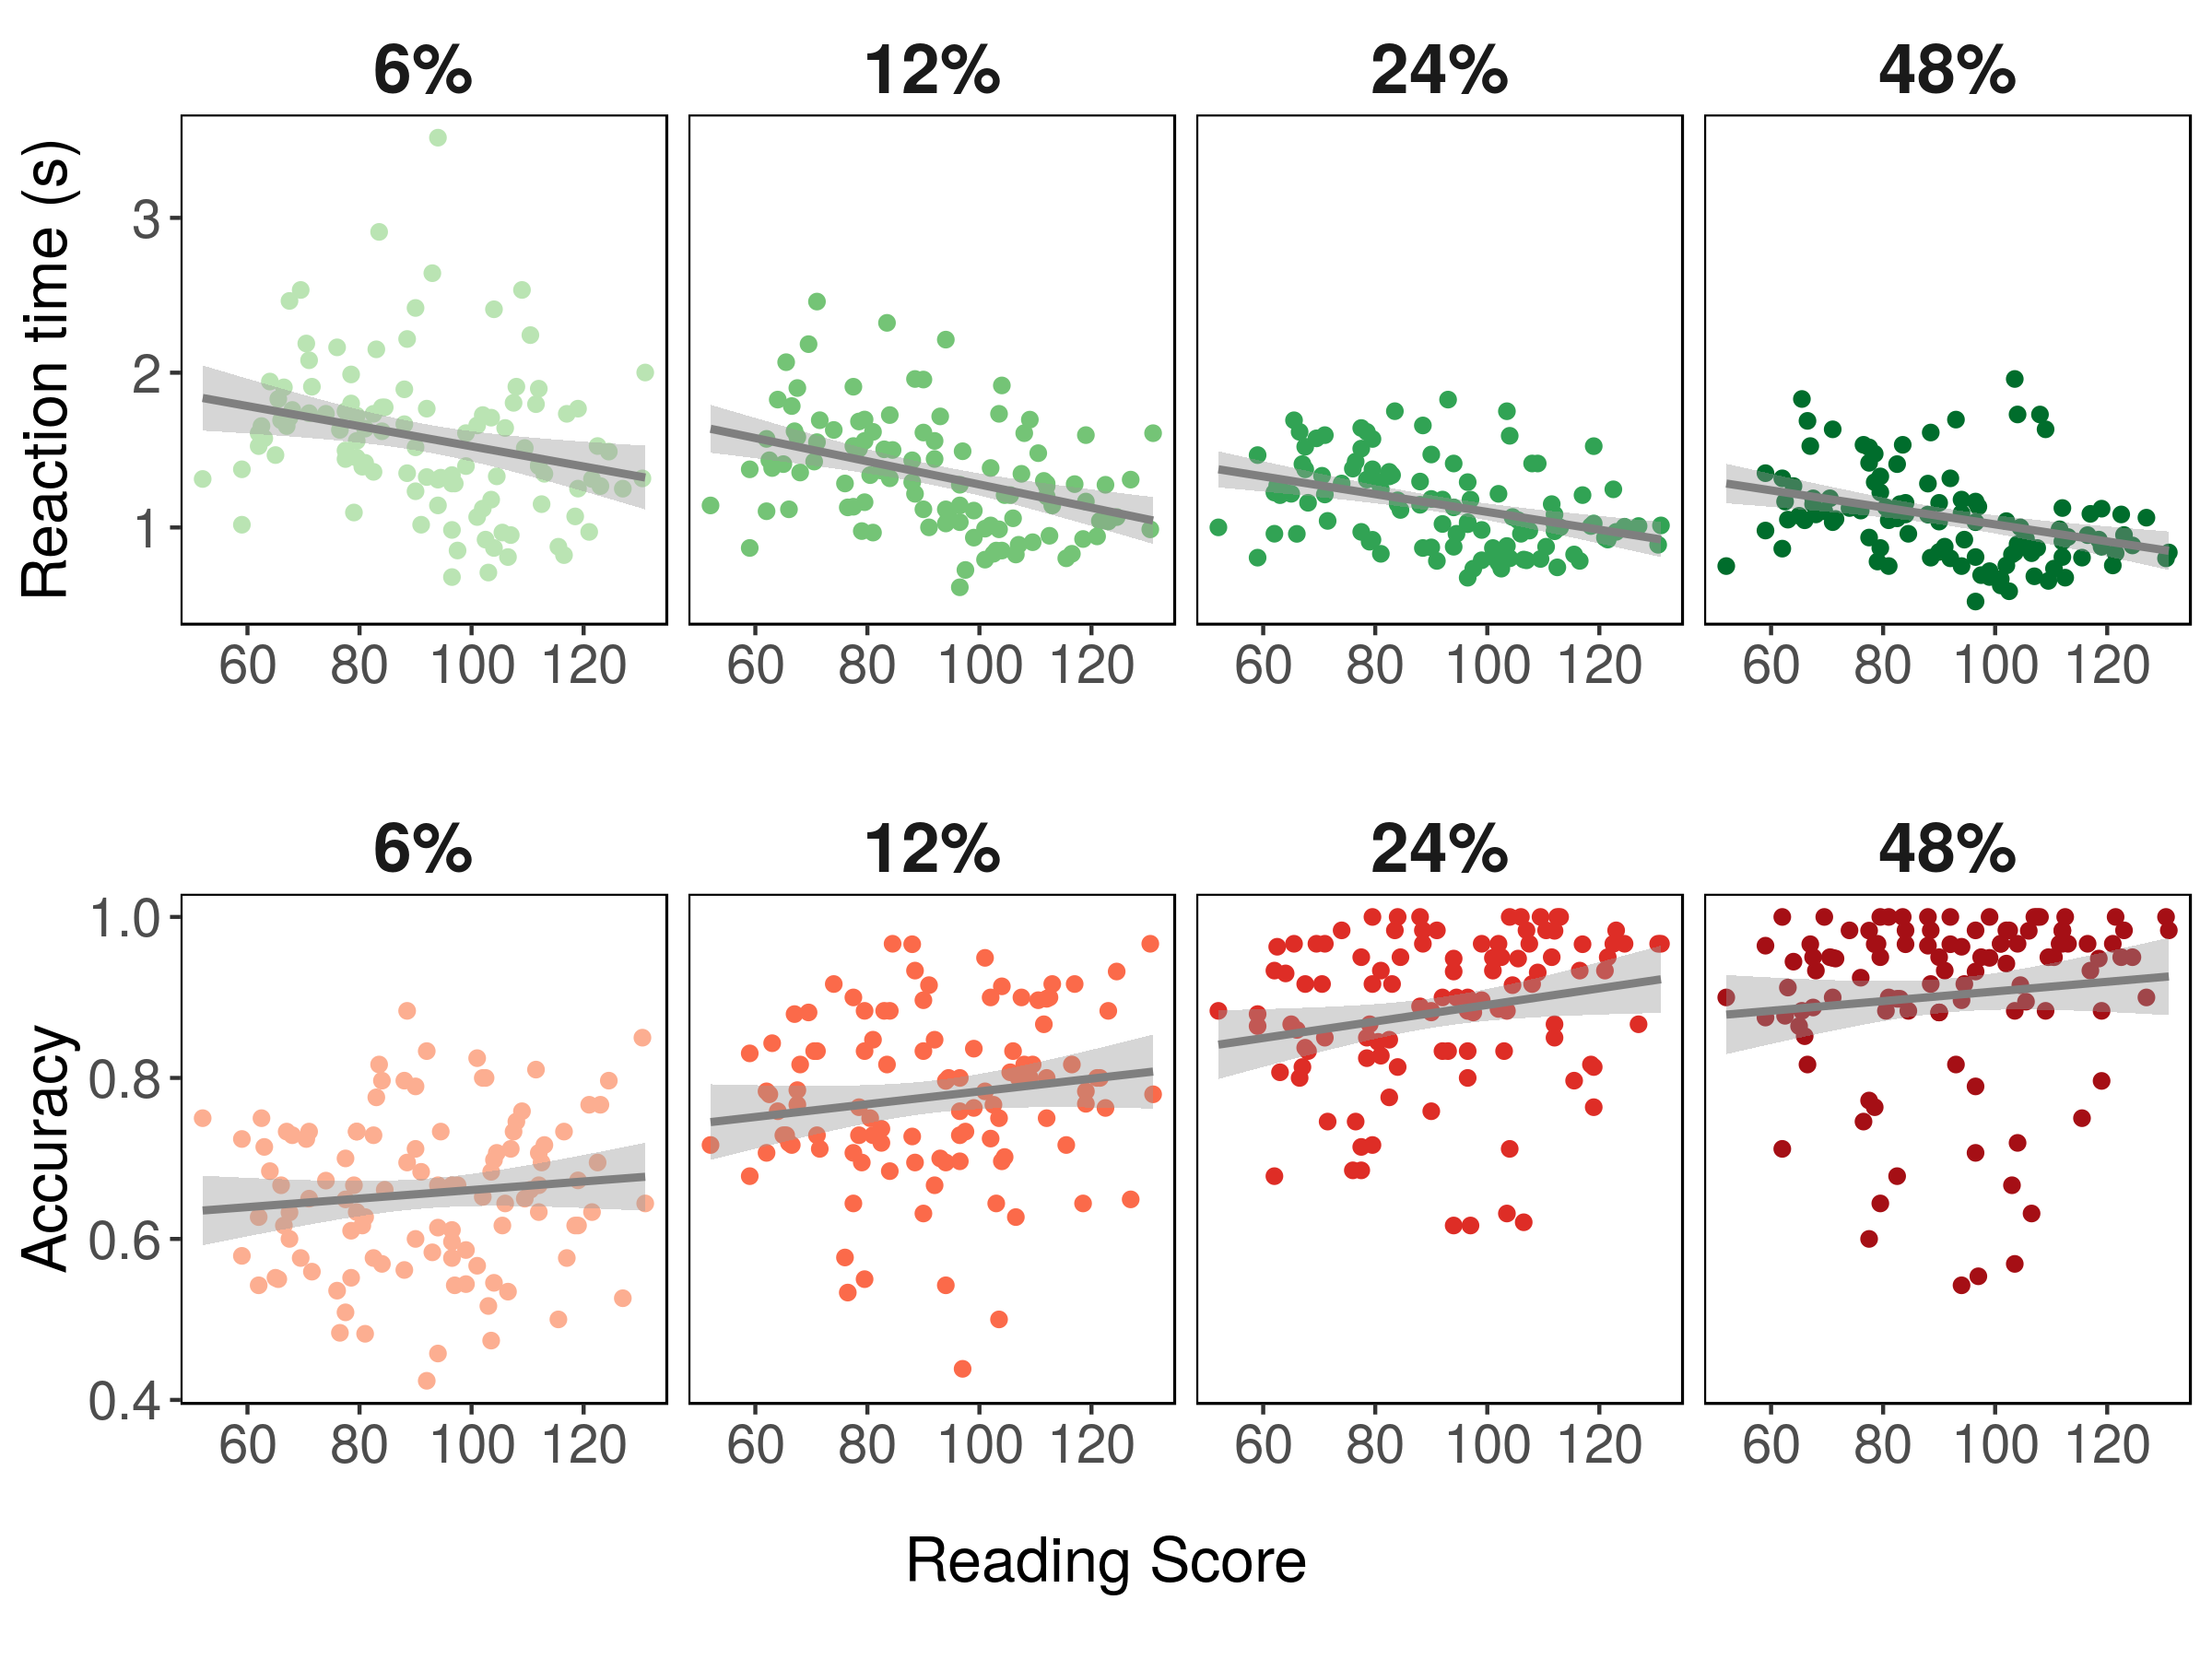
\includegraphics[width = 16 cm]{images/appendix_b/S1_Figure.png}
    \item \textit{Median reaction times (top row) and accuracy (bottom row) for each individual as a function of reading score. Panels show each stimulus coherence.}
\end{figure}

% FIGURE 2
\begin{figure}
    \centering
    \caption{Reaction time distributions for Control and Dyslexic groups.}
    \label{fig:suppb_2}
    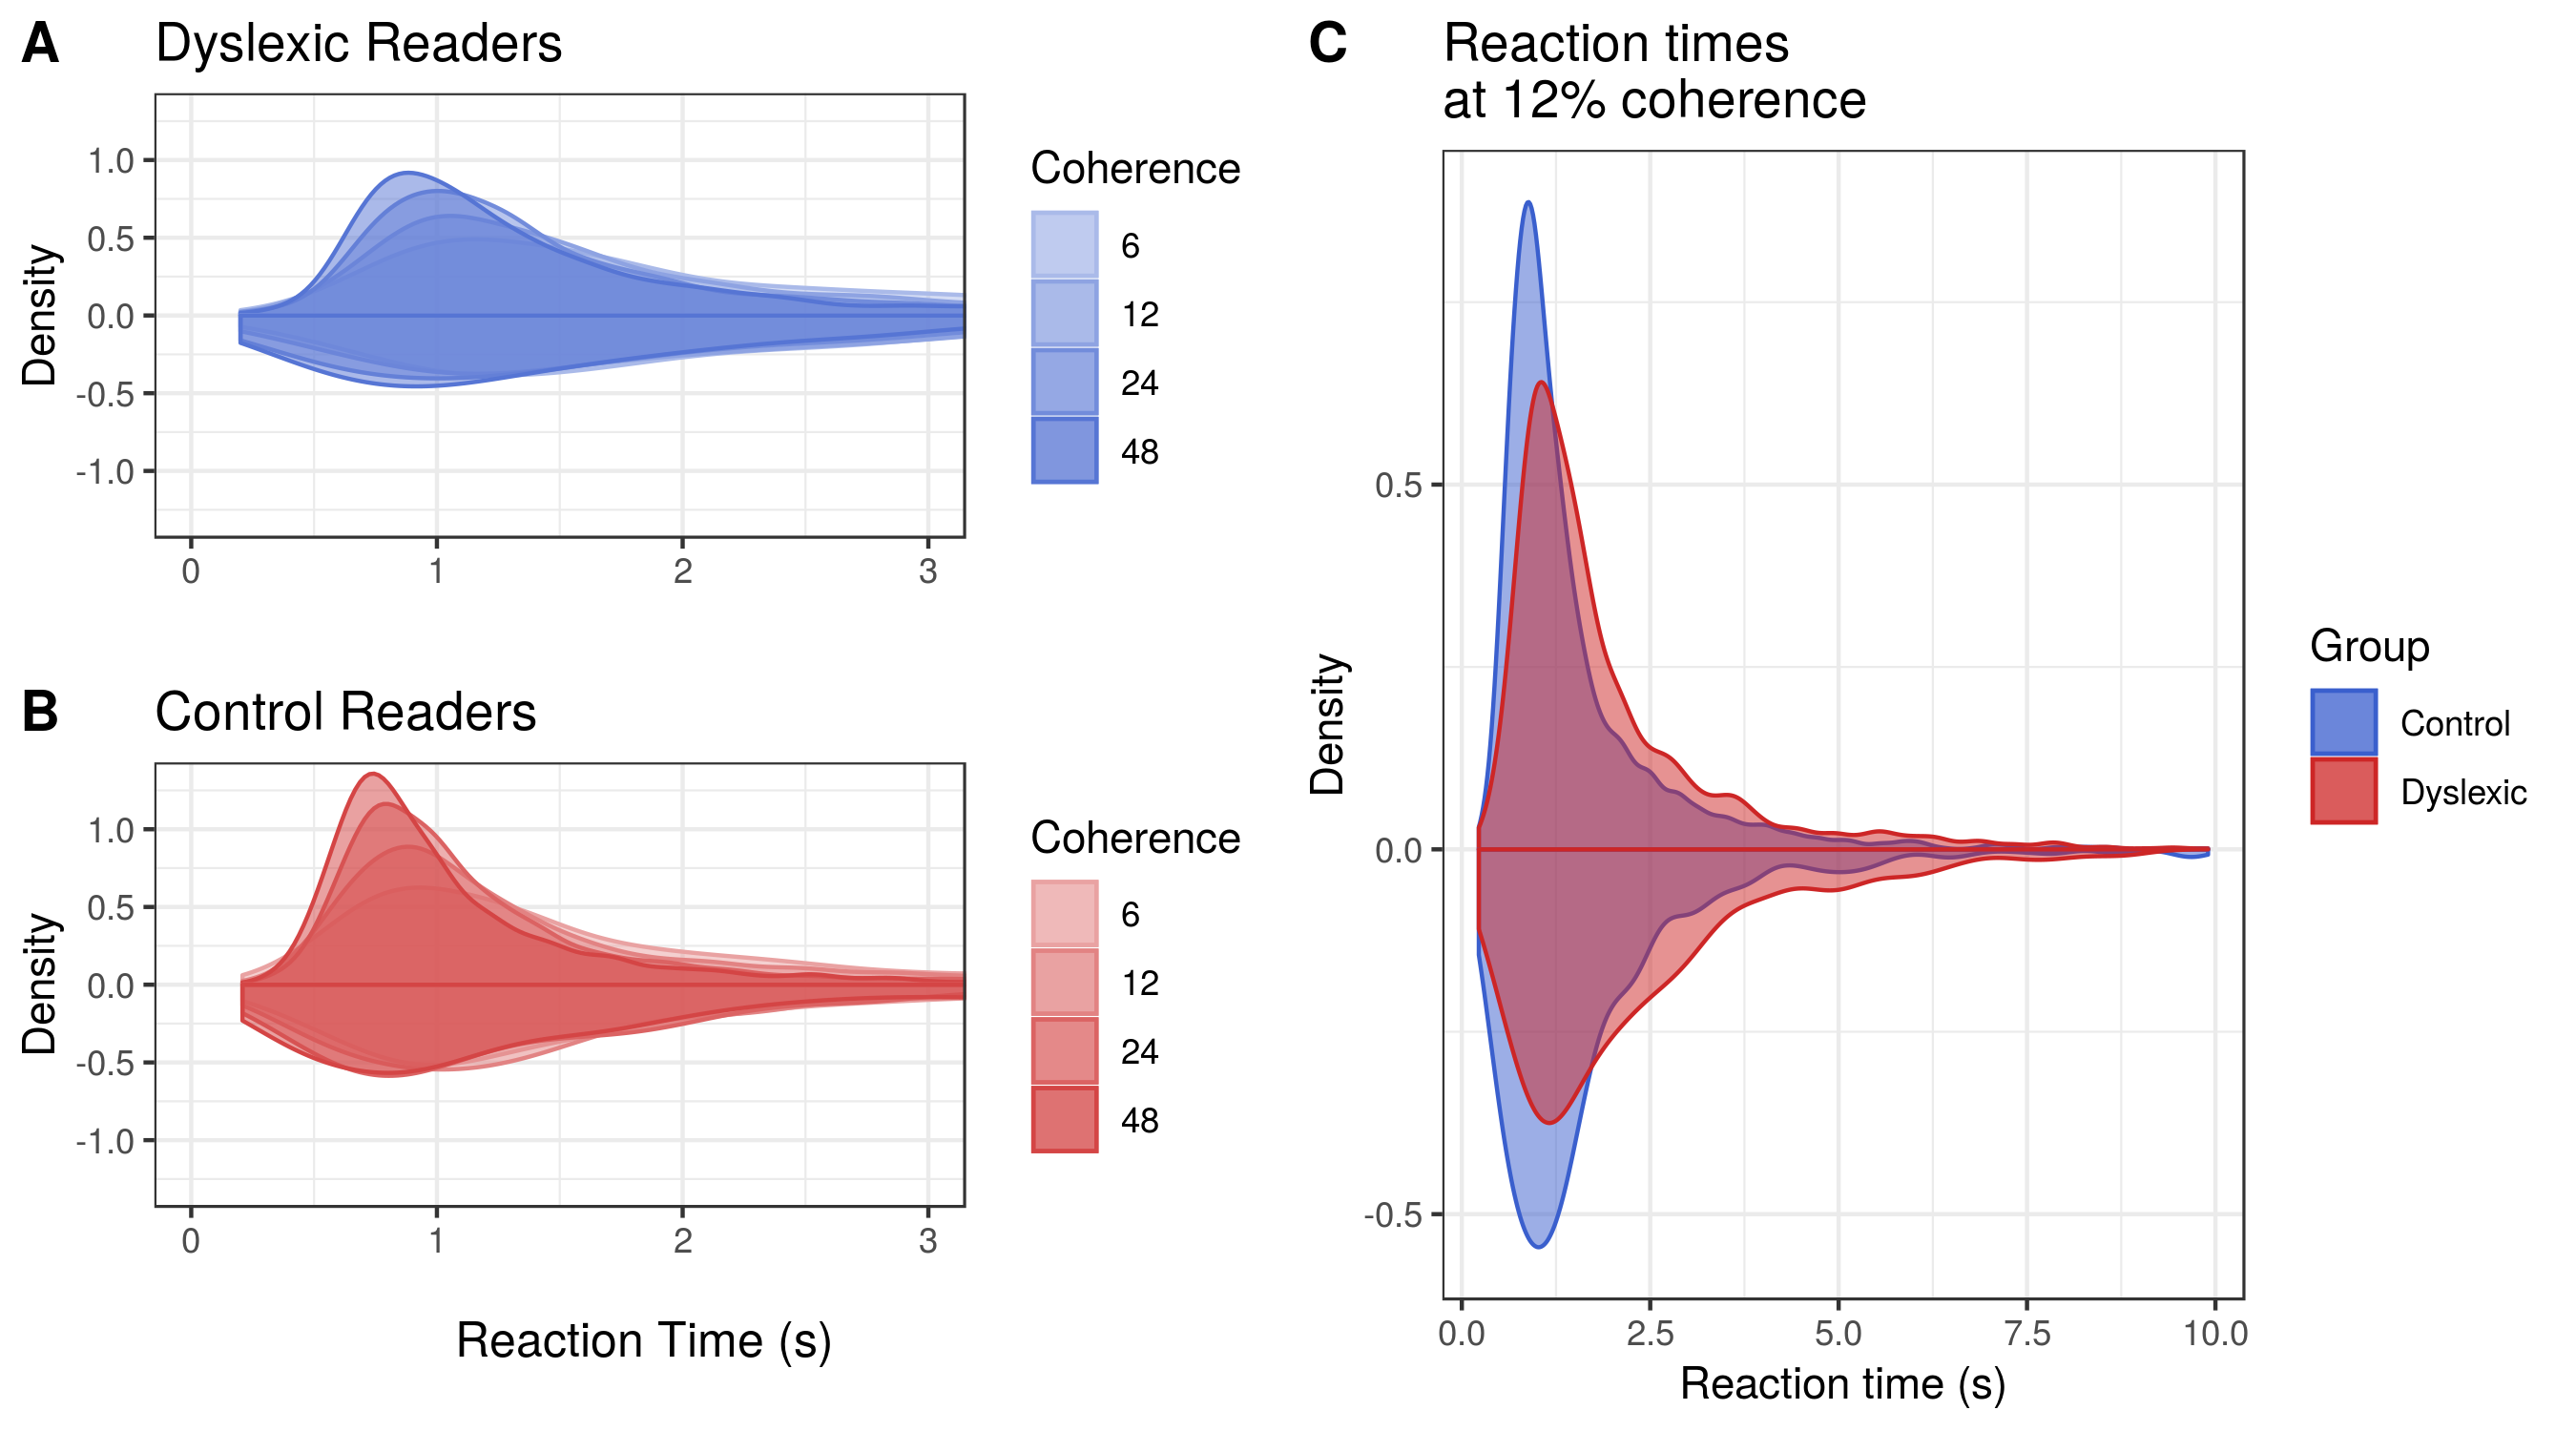
\includegraphics[width = 16 cm]{images/appendix_b/S2_Figure.png}
    \item \textit{Panels A-B: density plots of reaction times at each coherence level for the Dyslexic and Control groups. On the positive axis, correct response time distributions are shown, and on the negative axis error responses are shown. Plots are truncated at 3 seconds for ease of viewing. Panel C: overlaid density plots of reaction times at 12\% coherence for the Dyslexic and Control groups.}
\end{figure}

\section{Supplemental Analysis: group level statistics}
\subsection{Drift rate} As in the main manuscript, we used mixed model selection to identify the most parsimonious model of drift rate. Subject was included as a random effect, as our data contained four drift rate estimates per participant (one at each coherence level). The selected model included significant main effects of stimulus coherence and age, plus a significant interaction of stimulus coherence and group (Table~\ref{tab:sb_grpdrift}). The main effect of group was not significant ($p = 0.117$), but the direction of the relationship was the same as in the model where reading is treated as a continuous variable. Therefore, our results from both models are in qualitative agreement. The fact that reading skill was a significant main effect as a continuous measure but not as a discrete one is likely the result of reduced statistical power: there are 90 subjects in the group analysis, but 104 in the continuous-measure analysis. 

\begin{table}
\centering
\caption{Selected model of drift rate}
\label{tab:sb_grpdrift}
    \begin{tabular}{lrrl}
    \toprule
      & $\beta$ & SE & $p$\\
    \midrule
    (Intercept)      & 1.630  & 0.097 & $<$ 0.001\\
    Coherence        & 0.772  & 0.027 & $<$ 0.001\\
    Age              & 0.240  & 0.072 & 0.002\\
    Group            & -0.227 & 0.143 & 0.117\\
    Coherence:Group  & -0.133 & 0.053 & 0.014\\
    \bottomrule
    \end{tabular}
\end{table}

\subsection{Decision criterion parameters} The parameter $a$, representing an individual’s threshold of evidence for initiating a decision, was modeled as the dependent variable next. Linear mixed model selection dropped all three covariates, leaving only a main effect of group ($\beta = 0.351$, SE = 0.130, $p = 0.009$). 

The parameter $sz$, representing trial-to-trial variability in the drift process starting point, was modeled similarly. The selected model contained only a main effect of group, although this effect missed the standard threshold of significance ($\beta = 0.105$, SE = 0.060, $p = 0.085$).

\subsection{Non-decision time parameters} The selected model for residual non-decision time $t$ contained three main effects: group, nonverbal IQ and age, of which only group fell below the standard threshold of significance (Table~\ref{tab:sb_grpt}). 

Lastly, we considered the trial-to-trial variability in non-decision time st. The selected model contained two predictors: group and age at testing (Table S6). 

We can therefore see that the relationships between estimated DDM parameters and reading skill are qualitatively consistent regardless of whether reading disability is treated as a categorical or continuous variable. 
 
 
\begin{table}
\centering
\caption{Selected model of residual time $t$}
\label{tab:sb_grpt}
    \begin{tabular}{lrrl}
    \toprule
      & $\beta$ & SE & $p$\\
    \midrule
    (Intercept)      & 0.459  & 0.025 & $<$ 0.001\\
    Group            & 0.092  & 0.039 & 0.021\\
    Nonverbal IQ     & 0.032  & 0.020 & 0.104\\
    Age              & -0.31 & 0.018 & 0.085\\
    \bottomrule
    \end{tabular}
\end{table}

\begin{table}
\centering
\caption{Selected model of trial-to-trial variability in residual time $st$}
\label{tab:sb_grpst}
    \begin{tabular}{lrrl}
    \toprule
      & $\beta$ & SE & $p$\\
    \midrule
    (Intercept)      & 0.280  & 0.042 & $<$ 0.001\\
    Group            & 0.185  & 0.062 & 0.004\\
    Age              & -0.064 & 0.031 & 0.041\\
    \bottomrule
    \end{tabular}
\end{table}


% FIGURE 3
\begin{figure}
    \centering
    \caption{Lasso regression mean squared error as a function of regularization.}
    \label{fig:suppb_3}
    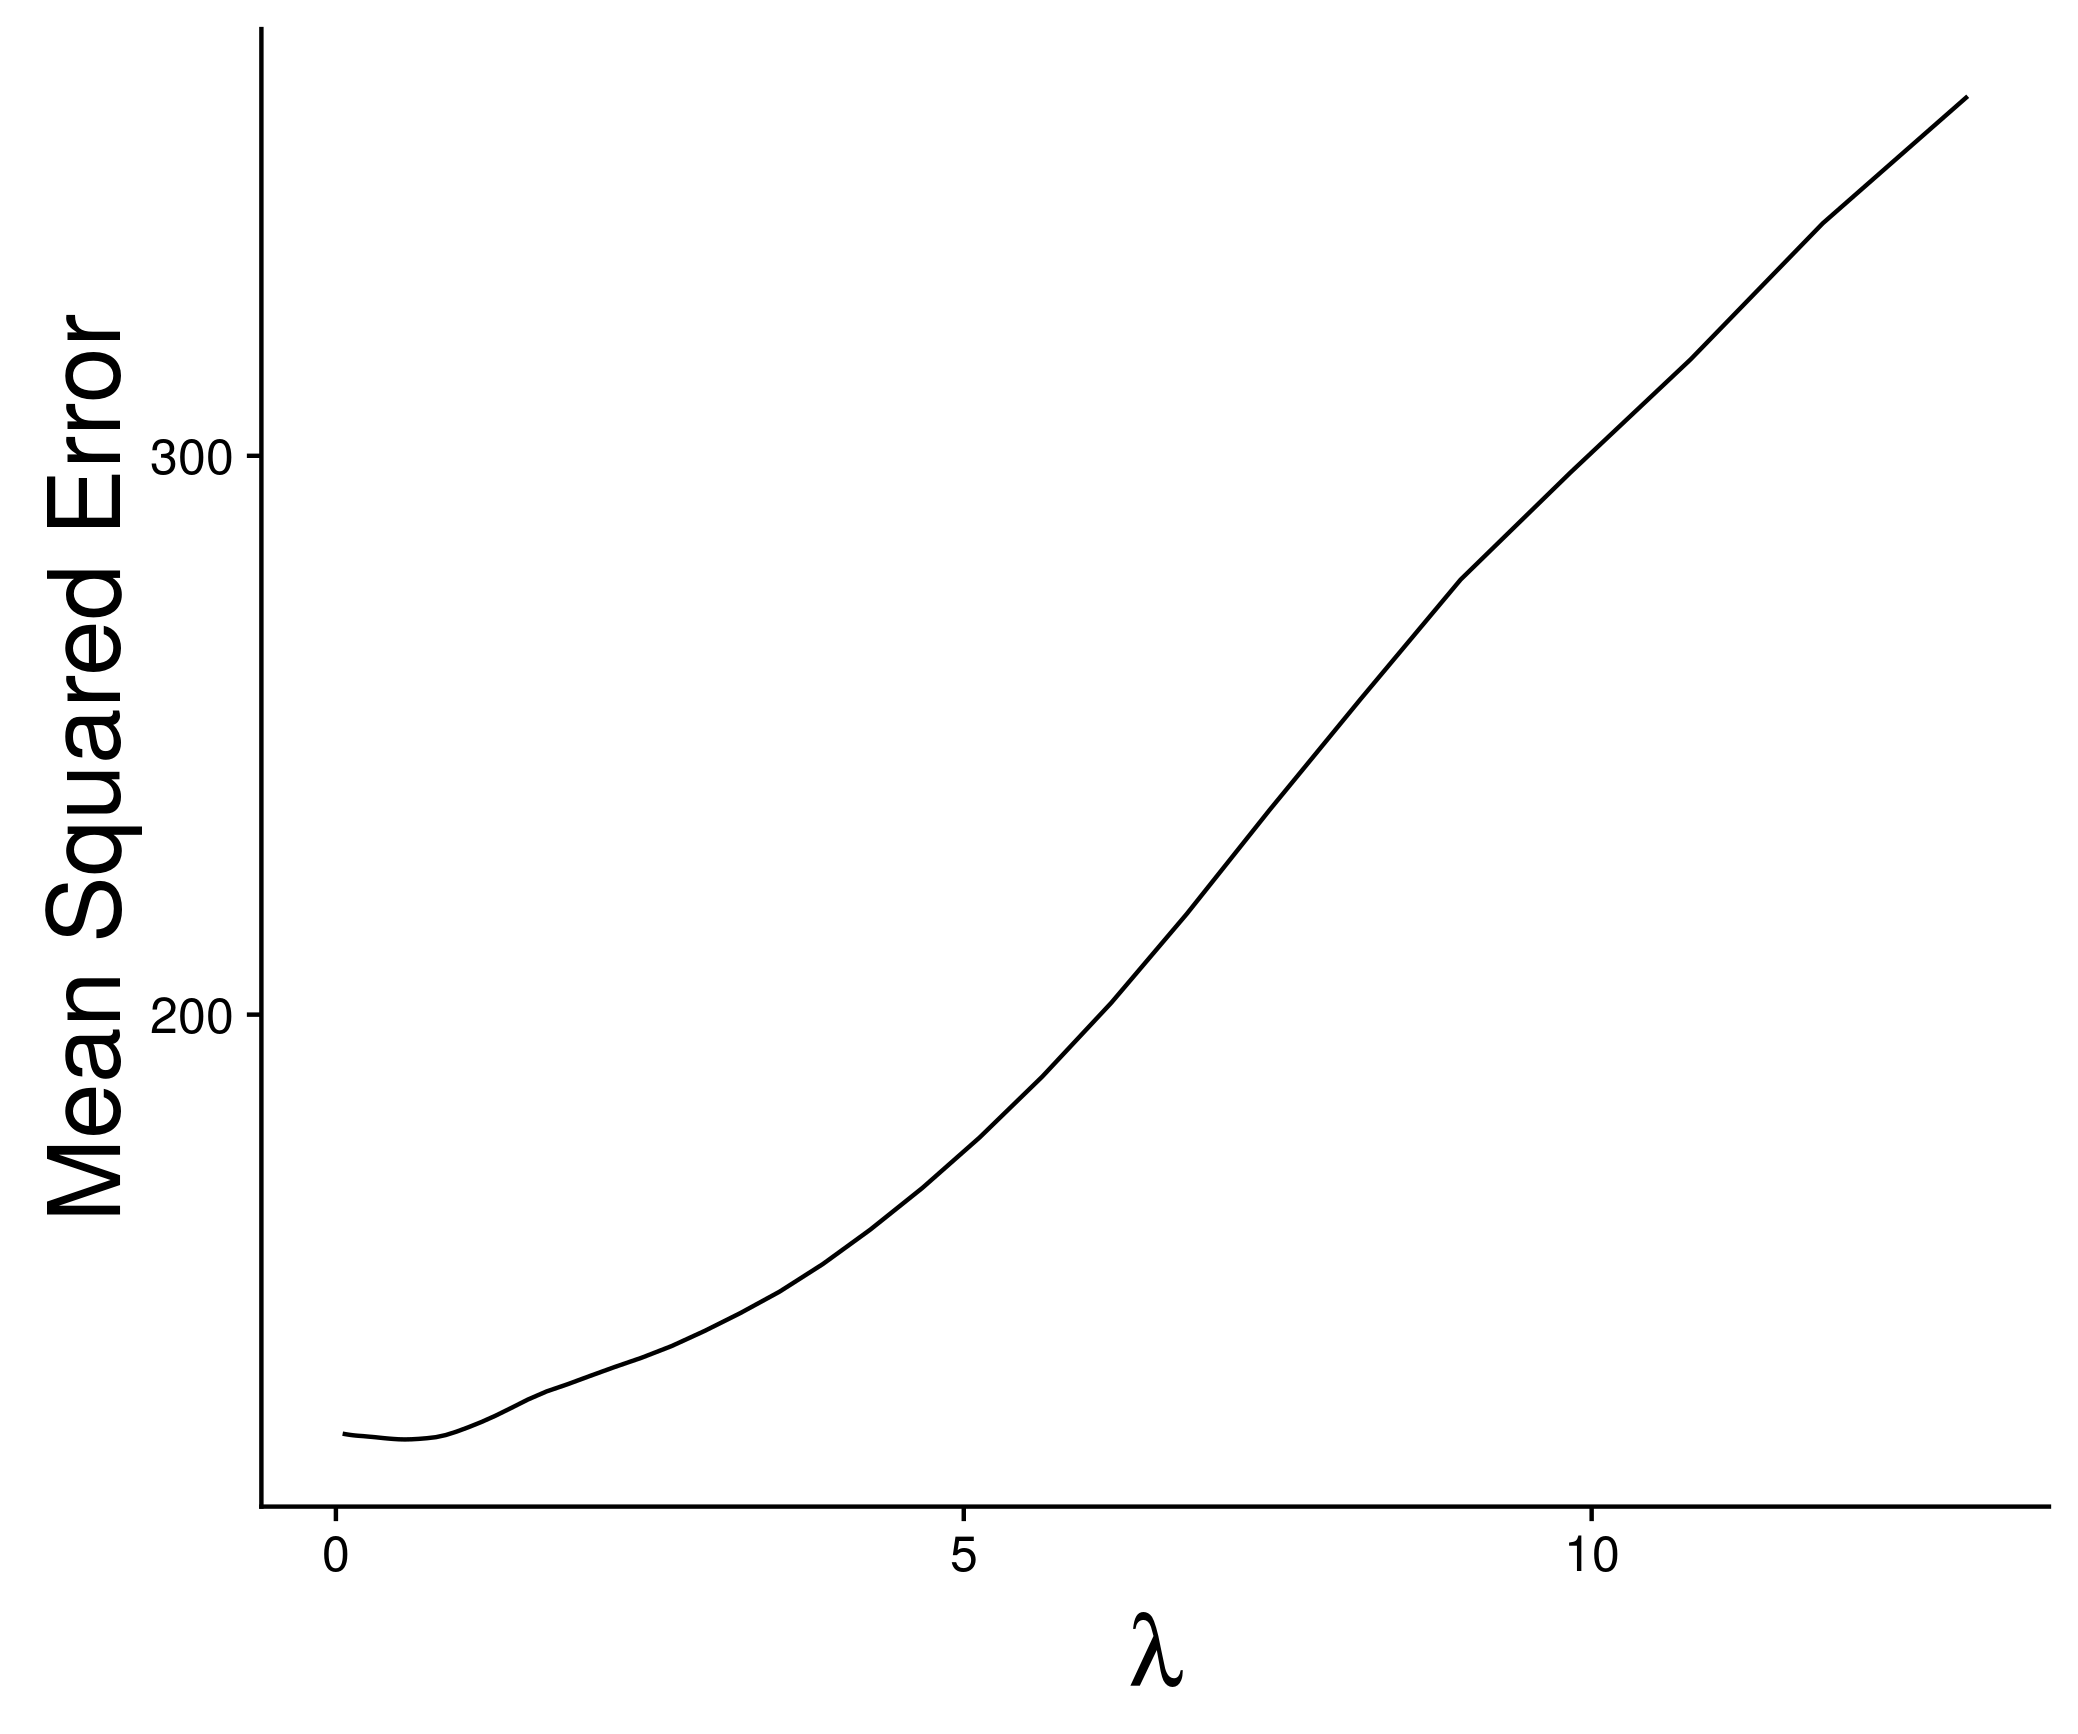
\includegraphics[width = 12 cm]{images/appendix_b/S3_lasso_MSE.png}
    \item \textit{Mean squared error (MSE) of lasso regression as a function of the regularization parameter $\lambda$ with 10-fold cross validation.}
\end{figure}

% FIGURE 4
\begin{figure}
    \centering
    \caption{Number of predictors retained by lasso regression as a function of regularization.}
    \label{fig:suppb_4}
    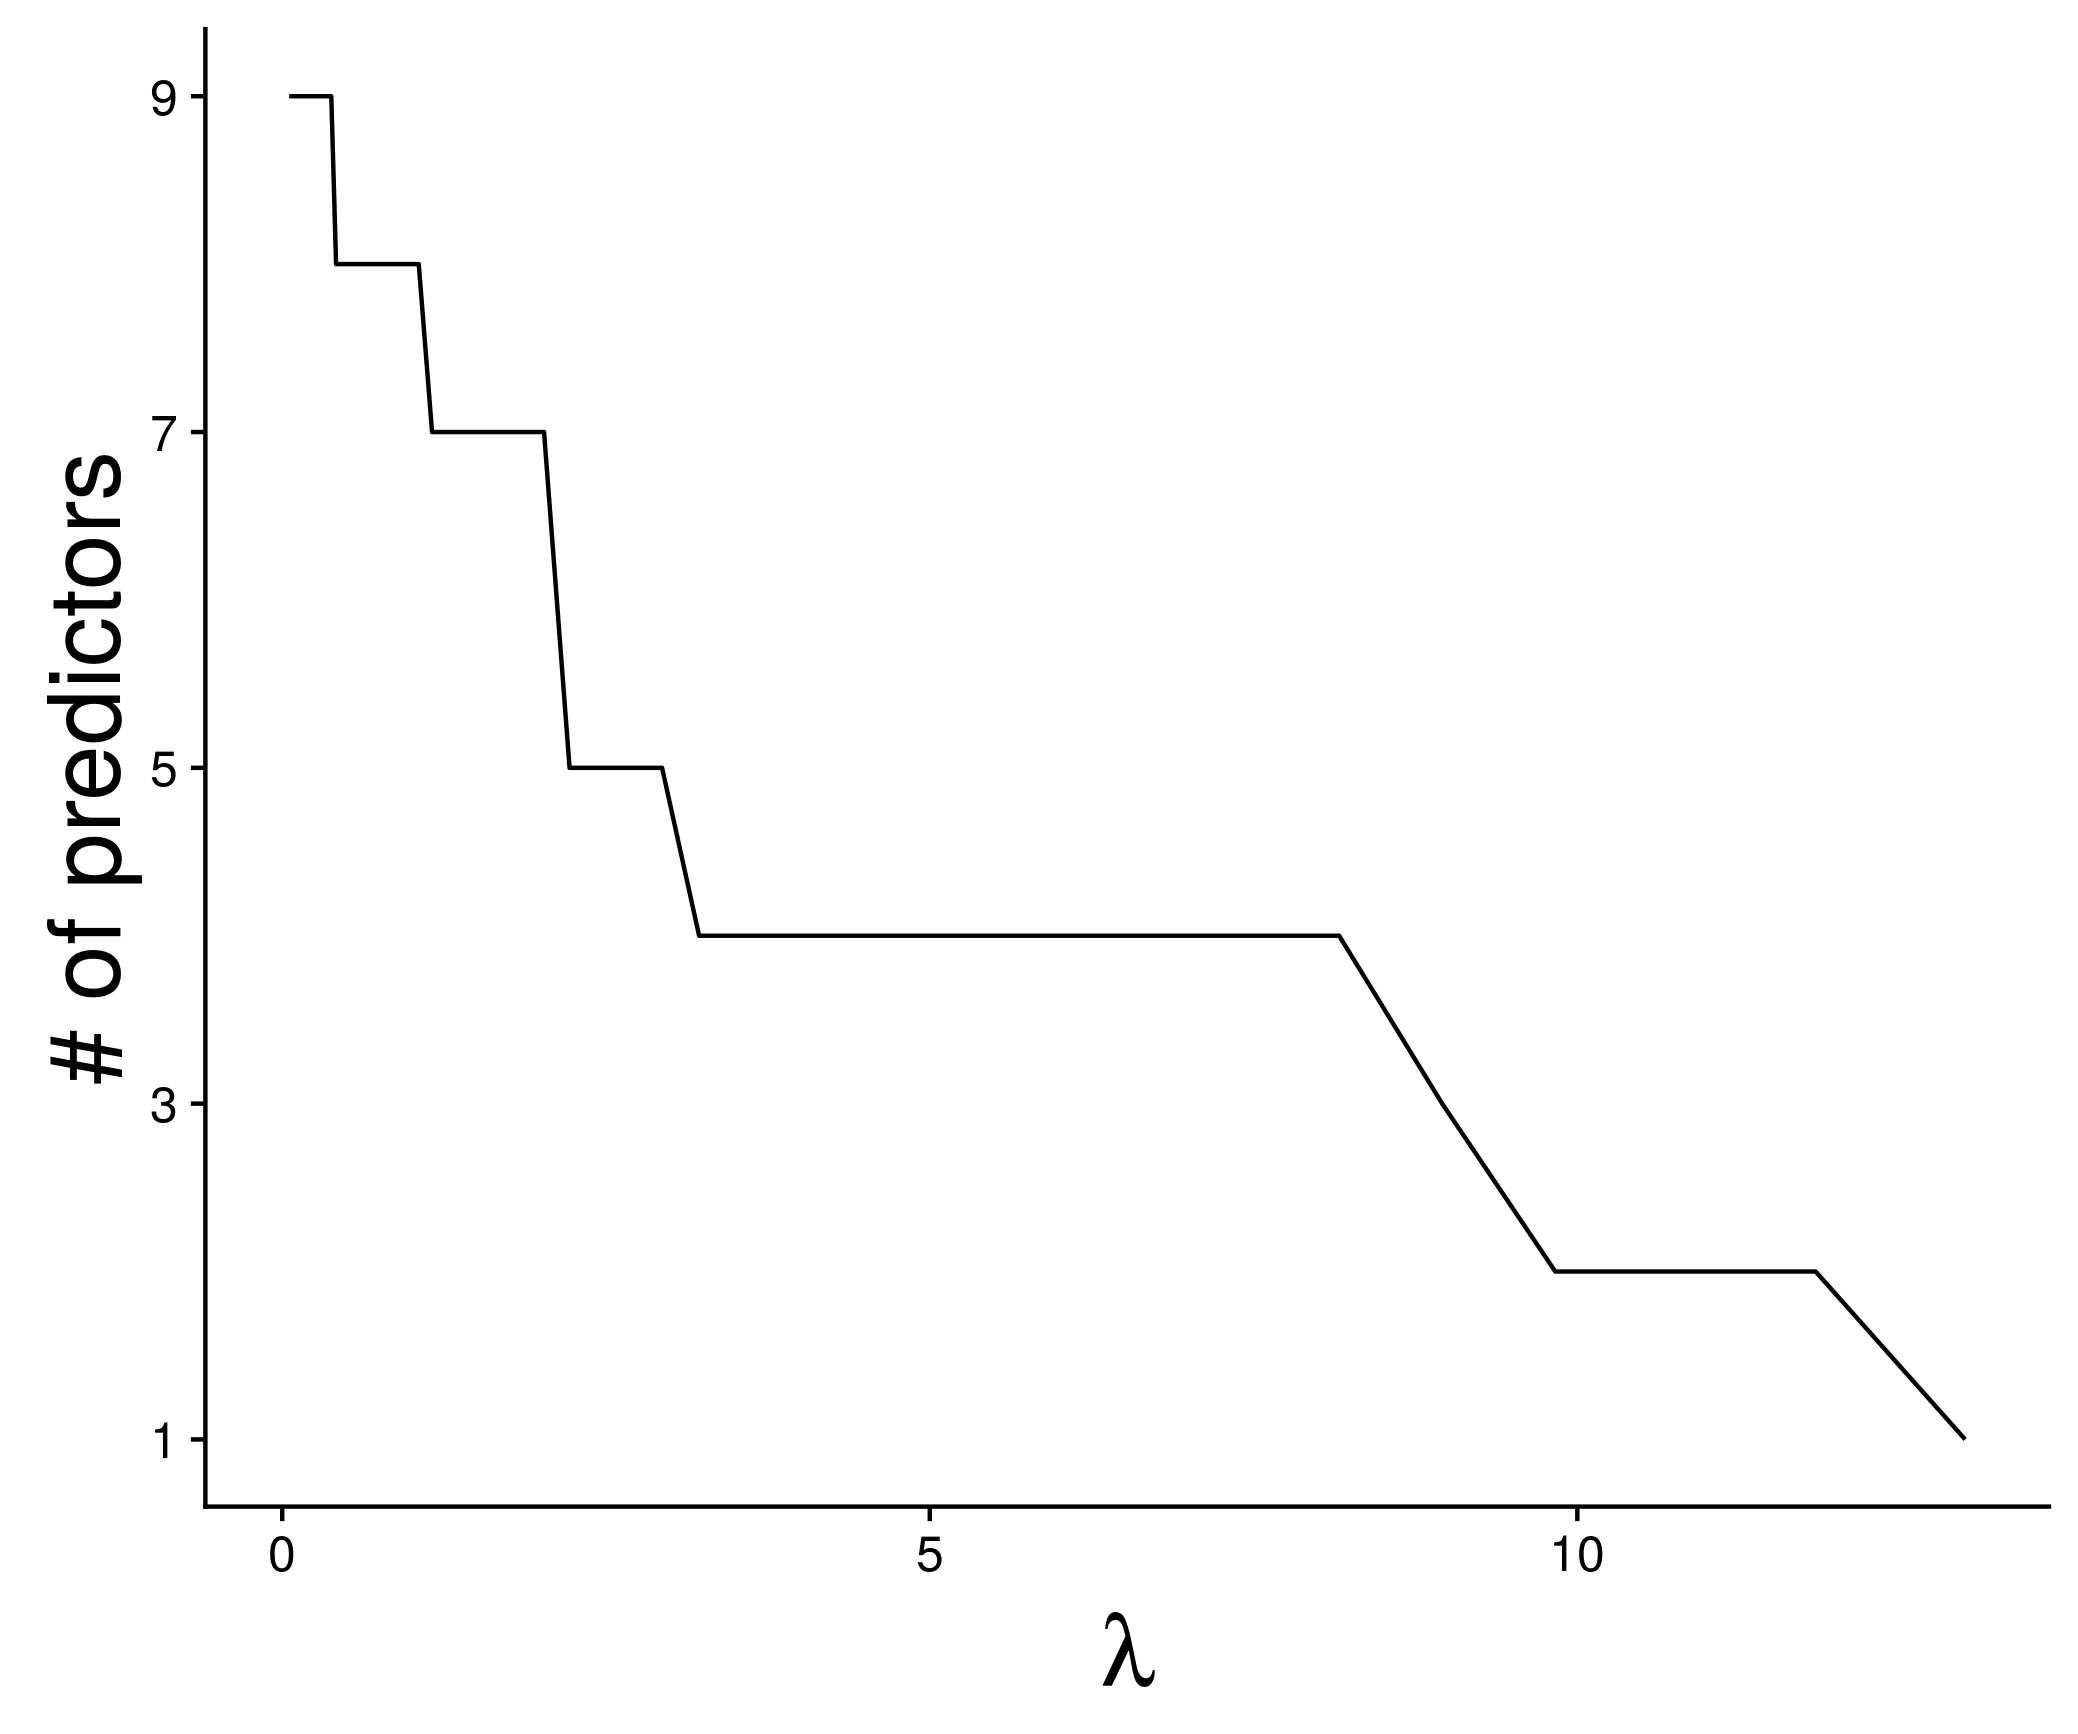
\includegraphics[width = 12 cm]{images/appendix_b/S4_lasso_npredictors.png}
    \item \textit{Number of predictors retained by lasso regression as a function of the regularization parameter $\lambda$ with 10-fold cross validation.}
\end{figure}

\begin{table}
\centering
\caption{Lasso model of reading skill}
\label{tab:sb_lasso}
    \begin{tabular}{lr}
    \toprule
      & $\beta$\\
    \midrule
    (Intercept)      & -3.28e-16\\
    $a$              & -0.092\\
    $v_{comp}$       & -0.090\\
    $d_{comp}$       & 0.118\\
    Nonverbal IQ     & 0.317\\
    CTOPP RAN        & 0.512\\
    CTOPP PA         & 0.169\\
    ADHD             & -0.002\\
    \bottomrule
    \end{tabular}
\end{table}



% FIGURE 5
\begin{figure}
    \centering
    \caption{Scree test for exploratory factor analysis.}
    \label{fig:suppb_5}
    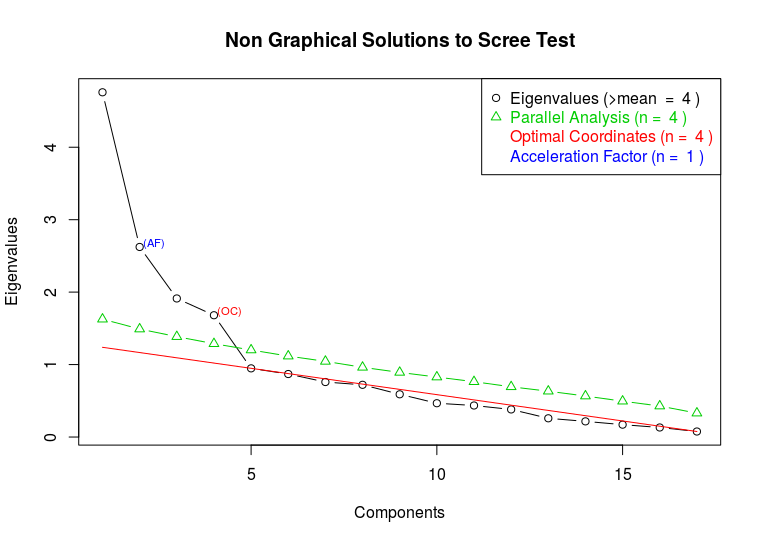
\includegraphics[width = 12 cm]{images/appendix_b/S5_scree_test.png}
    \item \textit{Scree test for exploratory factor analysis. Four standard measures of model fit are given: eigenvalues, parallel analysis, the optimal coordinates metric and acceleration factor metric.}
\end{figure}

% FIGURE 6
\begin{figure}
    \centering
    \caption{One-factor model predictions with cross-validation.}
    \label{fig:suppb_6}
    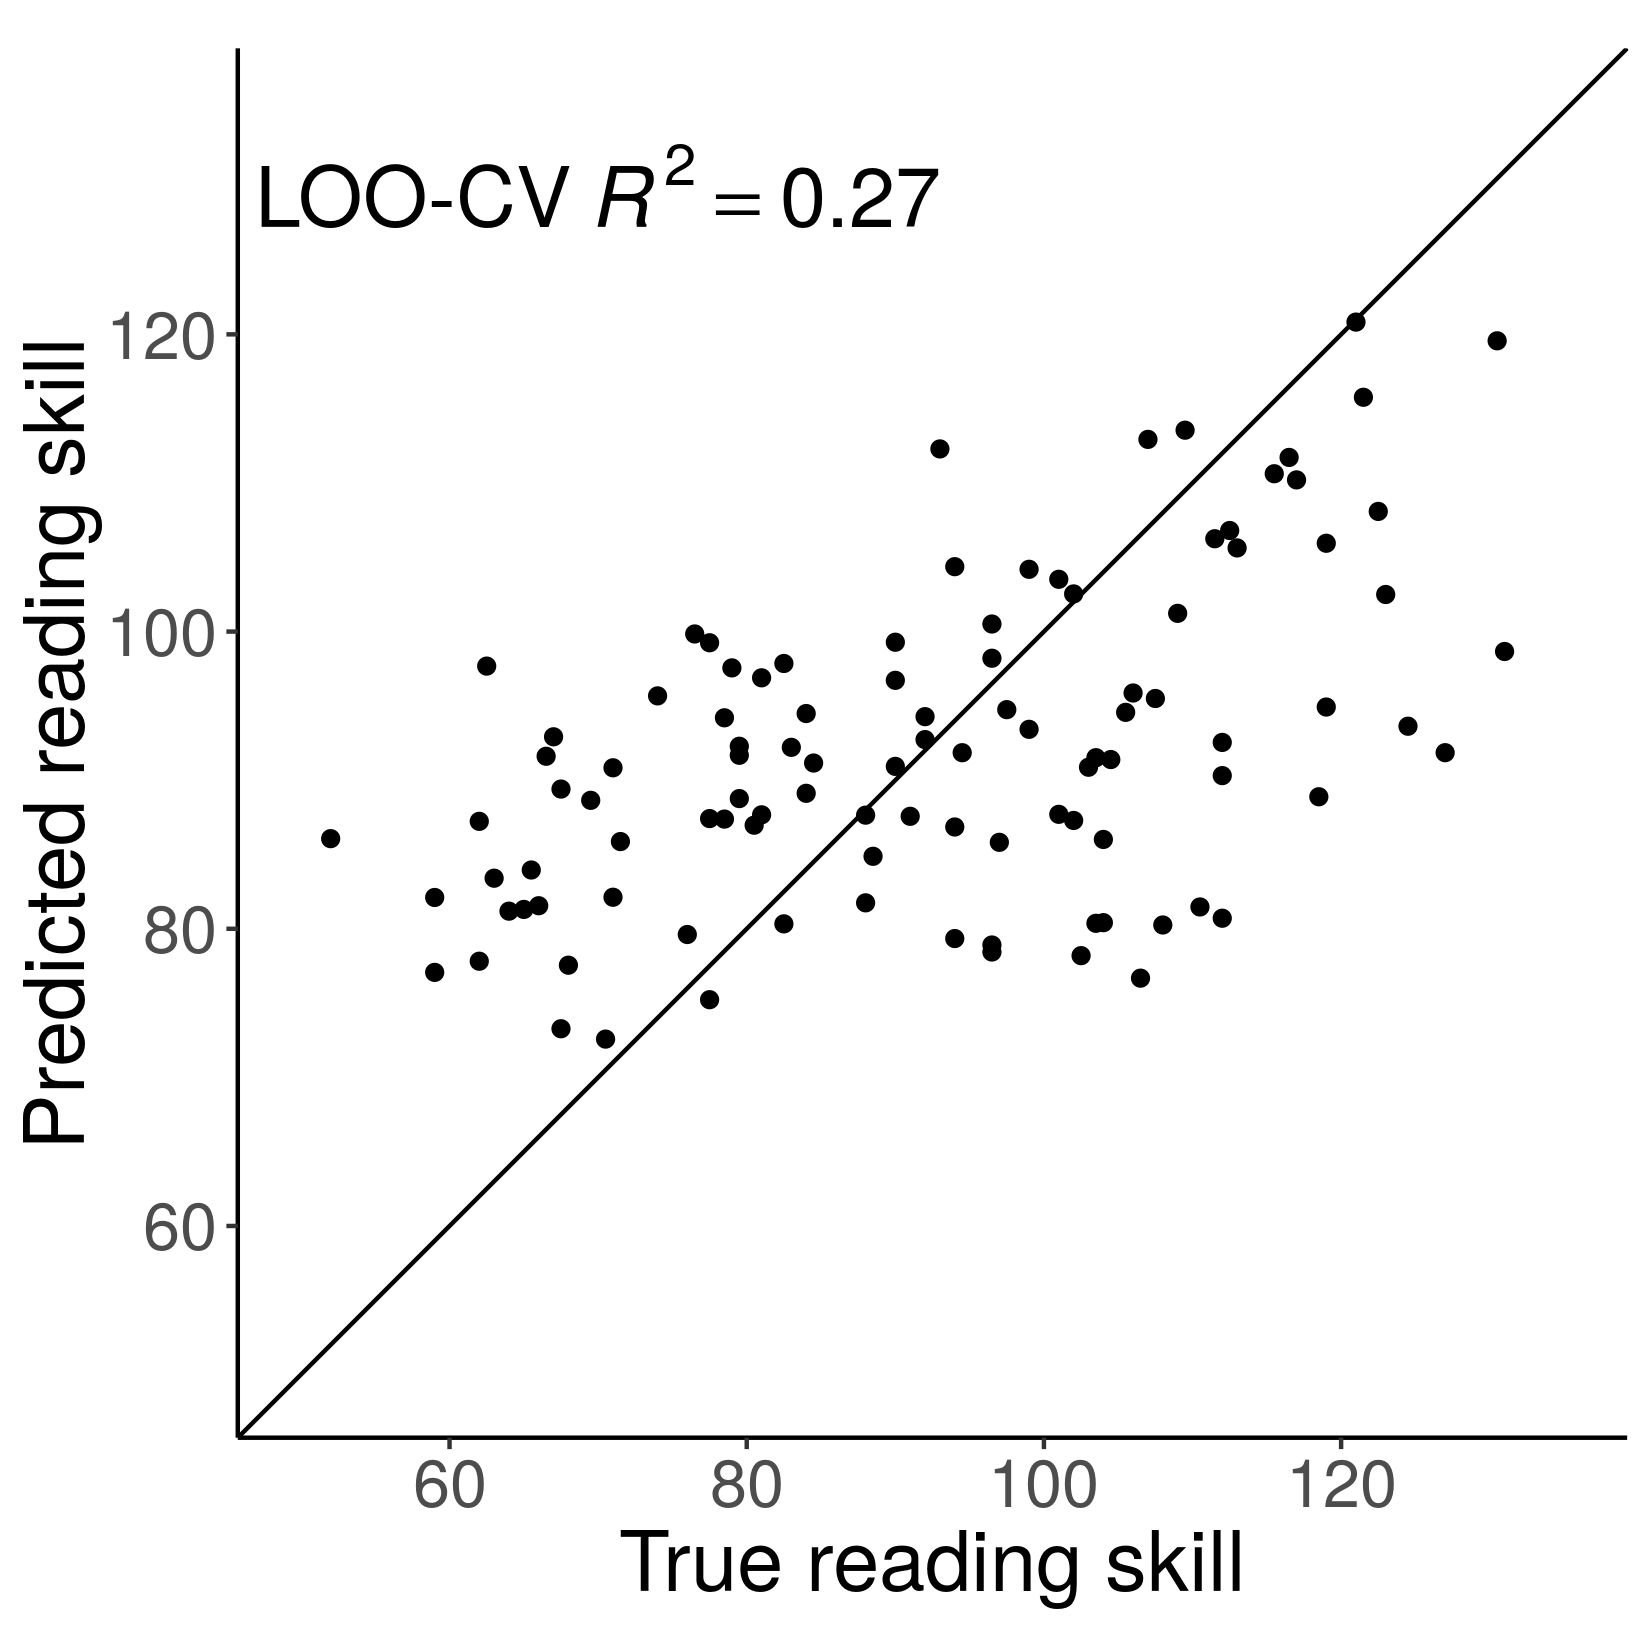
\includegraphics[width = 12 cm]{images/appendix_b/S6_DDM_model_1factor.png}
    \item \textit{Comparison of true versus predicted reading skill for the single-factor model. Point estimates are computed with leave-one-out cross validation (LOO-CV). }
\end{figure}




\end{document}